\documentclass[12pt]{article}
\usepackage{amssymb, amsthm, amsmath, amsfonts, fancybox, multicol, graphicx, 
type1cm, color, array, bardtex, verbatim, tikz, pgfplots}

\usetikzlibrary{shapes, shapes.geometric, positioning, automata, arrows.meta, 
calc}

\tikzset{
	simplex/.pic={
		\newcount\mycount
		\tikzset{state/.style={fill=none, draw=violet, text=black, 
		shape=circle}}
		\pgfmathsetmacro\rot{360.0/\N}
		\begin{scope}[rotate=\rot]
			\node[regular polygon, regular polygon sides=\N,
				minimum size=\radius, rotate=\rot] (A) {};
			\pgfmathsetmacro\None{\N-1}
			\foreach \i in {1,...,\N}
			\node[state] (\i) at (A.corner \i) {\i};
			
			\foreach \i in {1,...,\None}{
				\mycount=\i
				\advance\mycount by 1
				\foreach \j in {\the\mycount,...,\N} {
					\draw[-{Stealth[scale=1.5,angle'=45]},semithick] (\i) -- (\j);
				}
			}
		\end{scope}
	},
	N/.store in=\N,
	radius/.store in=\radius,
	radius=10cm,
	N=5,
}

\graphicspath{{resources/}}

\styleoption{poster}
\posterstyle{stylefour}
\toptitlecolor{Fuchsia}
\boxcolor{Thistle}
\boxtitlecolor{Periwinkle}

\begin{document}

\begin{posterbard}

	%\postertopwidthfactor{5}
	\postertopscale{Neural Network Reconstruction via Graph Locality-Driven 
		Machine Learning}{Hayden Sartoris}{Computer Science}{May 2018}{Sven 
	Anderson, Arseny Khakhalin}{2}

	\fontsize{\boxfontsize}{1.2\boxfontsize} \selectfont
	\setlength{\columnseprule}{0pt}
	\setlength{\columnsep}{0.01\textwidth}

	\begin{posterboxtitle}{Overview}
		\noindent We propose an algorithm inspired by convolutional approaches 
to image processing, adapted to the graph structure of neural networks, in order 
to solve the problem of network reconstruction from spiking data.
To achieve this, we redefine locality in terms of graph adjacency, and create a 
scale-independent algorithm facilitated by modern machine learning techniques to 
incorporate this locality data into individual connection prediction.
	\end{posterboxtitle}

	{\boxtitlecolor{PineGreen}
	\begin{posterboxtitle}{Process}
		\noindent Our goal was to infer biological neural network connectivity 
		from spiking data. To do so, we created the following data pathway:
		\begin{center}
			\scalebox{1.1}{
			\begin{tikzpicture}[node distance=5em,->,
				-{Stealth[scale=1.5,angle'=45]},semithick]
				\tikzset{state/.style={fill=none, draw=black, text=black,
					shape=circle}}
				\node[state] (0) {0};
				\node[state] (1) [right of=0] {1};
				\node[state] (2) [below right of=0] {2};

				\path 	(0) edge node {} (1)
						(0) edge node {} (2)
						(1) edge node {} (2);
				\node (arrow) [below right=1.3cm of 1] 
					{\scalebox{1.5}{$\Rightarrow$}};
				\node (gen_1) [left=6cm of arrow, align=left] 
				{Generator\\network};
				\node (input) [right=1cm of arrow] 
					{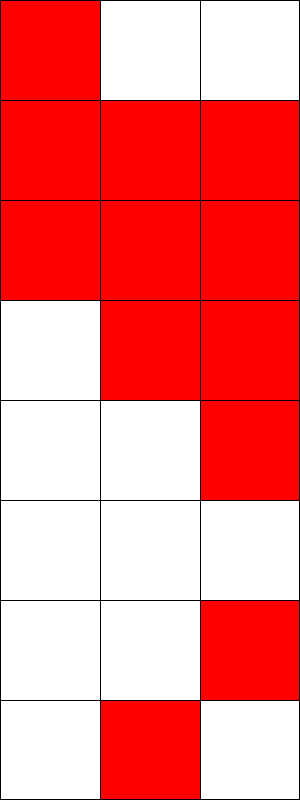
\includegraphics[width=.07\textwidth]{fullRun/0_py/input.png}};
				\node (spike) [right=1.8cm of input, align=left] 
				{Spiking\\data};
				\node (arrow2) [below=.8cm of input] 
					{\rotatebox{-90}{\scalebox{1.5}{$\Rightarrow$}}};
				\tikzset{state/.style={shape=rectangle, draw=black, minimum 
				height=4cm, minimum width=4cm}}
				\node[state] (model) [below=.8cm of arrow2] {Model};
				\node (proc) [right=1cm of model, align=left] {Processing};
				\node (arrow3) [left=.6cm of model] 
					{\scalebox{1.5}{$\Leftarrow$}};
				\tikzset{state/.style={fill=none, draw=black, text=black,
					shape=circle}}
				\node[state] (3) [below=7.5cm of 0] {0};
				\node[state] (4) [right of=3]{1};
				\node[state] (5) [below right of=3] {2};

				\path 	(3) edge node {} (4)
						(3) edge node {} (5)
						(4) edge node {} (5);

				\node (gen2) [below=7.5cm of gen_1, align=left] 
					{Generator\\structure};

			\end{tikzpicture}}
		\end{center}
		%\begin{enumerate}
		%	\item Considered biological networks in terms of a graph 
		%		representation
		%	\item Identified features within that graph representation 
		%		potentially useful to reconstruction
		%	\item Created a model based around an algorithm informed by these 
		%		features and inspired by convolutional neural networks
		%	\item Generated data from a variety of simple test networks
		%	\item Trained models on that data and analyzed the resulting output 
		%		to determine efficacy
		%\end{enumerate}
	\end{posterboxtitle}}

	\begin{posterbox}
		\begin{center}\textbf{Spike-time Raster Plots}\end{center}
		For a three neuron network sampled for eight timesteps, a raster plot 
		might appear as below.\\
		\vspace{1em}
		\begin{center}
			\begin{tikzpicture}
			\node (input) 
				{\scalebox{.2}{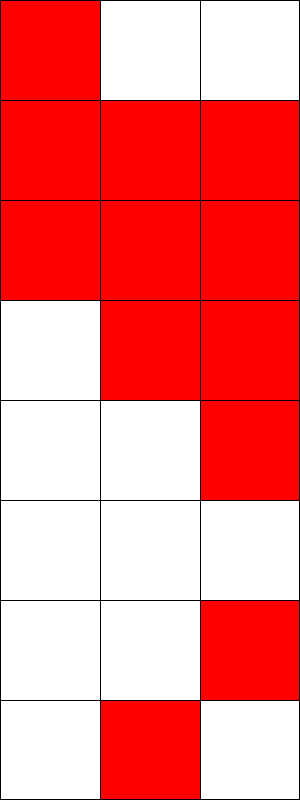
\includegraphics[width=\textwidth]{fullRun/0_py/input.png}}};
			\node (neurons) [above=.7cm of input] {\textit{neurons} 
			$\rightarrow$};
			\node (time) [left=1cm of input] {\rotatebox{90}{$\leftarrow$ 
				\textit{time}}};
			\node (label1) [below=1cm of input, align=center] {Produced by\\
				{\color{red}training} network};

			\node (input2) [right=7cm of input]
				{\scalebox{.2}{
\includegraphics[width=\textwidth]{fullRun/invert/input.png}}};
			\node (neurons2) [above=.7cm of input2] {\textit{neurons} 
			$\rightarrow$};
			\node (time2) [left=1cm of input2] {\rotatebox{90}{$\leftarrow$ 
				\textit{time}}};
			\node (label2) [below=1cm of input2, align=center] {Produced by\\
				{\color{blue}inverted} network};
			\end{tikzpicture}
			
		\end{center}
		\vspace{\baselineskip}
	\end{posterbox}

	{\boxtitlecolor{CornflowerBlue}
	\begin{posterboxtitle}{Biological Networks \& Graphs}
		\noindent \textbf{Graph Representation of Neural Networks}
		\begin{itemize}
			\item Biological networks are broadly equivalent to directed graphs 
				(diGraphs)
			\item diGraphs consist of nodes and edges, as below
			\item In neural networks, neurons are nodes and connections are 
				edges
			\item Probability of connection between two neurons unrelated to 
				physical proximity
		\end{itemize}
		\begin{center}
			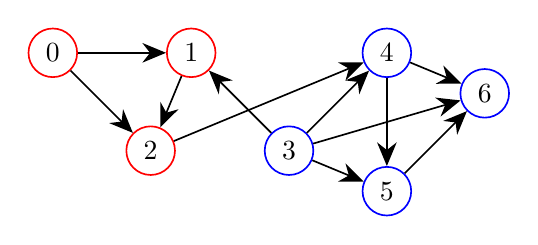
\begin{tikzpicture}[node distance=5em,->,
				-{Stealth[scale=1.5,angle'=45]},semithick]
				\tikzset{state/.style={fill=none, draw=red, text=black,
					shape=circle}}
				\node[state] (0) {0};
				\node[state] (1) [right of=0] {1};
				\node[state] (2) [below right of=0] {2};

				\path 	(0) edge node {} (1)
						(0) edge node {} (2)
						(1) edge node {} (2);
				
				\tikzset{state/.style={fill=none, draw=blue, text=black,
					shape=circle}}
				\node[state] (3) [right of=2] {3};
				\node[state] (4) [above right of=3] {4};
				\node[state] (5) [below of=4] {5};
				\node[state] (6) [above right of=5] {6};

				\path 	(3) edge node {} (4)
						(3) edge node {} (5)
						(3) edge node {} (6)
						(4) edge node {} (5)
						(4) edge node {} (6)
						(5) edge node {} (6);

				\path 	(3) edge node {} (1)
						(2) edge node {} (4);
			\end{tikzpicture}
		\end{center}
		\textbf{Common Local Structures}
		\begin{itemize}
			\item Motifs, repeating local structures, unusually common in 
				biological networks
			\item Some motifs, simplices, are structures in which information 
				flows in one direction, from a `source' node to a `sink' node
		\end{itemize}
		The graph above contains a 2-simplex, in red, and a 3-simplex, in blue.  
		Below, a 6-simplex, in {\color{violet}violet}.\\
		\vspace{1em}
		\begin{center}
			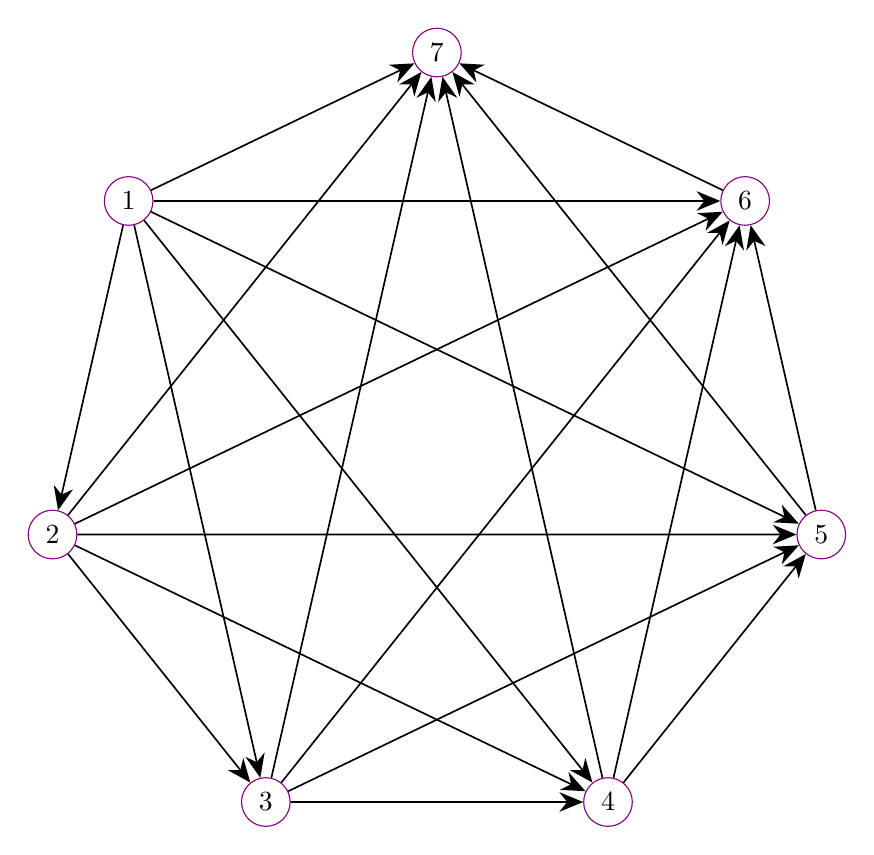
\begin{tikzpicture}
				\pgfmathsetmacro\N{7}
				\pic {simplex={N=\N}};
			\end{tikzpicture}
		\end{center}
		\vspace{1em}
	\end{posterboxtitle}
	}


	{\boxcolor{Melon}
	\begin{posterbox}
		\begin{center}\textbf{Graph Convolution}\end{center}
		Given that local structure is important to the functioning of biological 
		neural networks, providing locality information to an algorithm 
		performing reconstruction could aid that process.
		\begin{center}
		\begin{tikzpicture}[node distance=5em,->,
			-{Stealth[scale=1.5,angle'=45]},semithick]
			\tikzset{state/.style={fill=none, draw=black, text=black,
				shape=circle}}
				\node[state] (i) {i};
				\node[state] (j) [right=6cm of i] {j};
				\pgfmathsetmacro\dist{.1em}
				\node (k1) [above=\dist of j] {};
				\node (k2) [above right=\dist of j] {};
				\node (k3) [right=\dist of j] {};
				\node (k4) [below right=\dist of j] {};
				\node (k9) [below=\dist of j] {};

				\node (k5) [below=\dist of i] {};
				\node (k6) [above left=\dist of i] {};
				\node (k7) [left=\dist of i] {};
				\node (k8) [below left=\dist of i] {};
				\node (k10) [above=\dist of i] {};
				\path 	(j) edge node {} (i)
					%(k1) edge [bend left] node {} (j)
					(k2) edge [bend left] node {} (j)
						(k3) edge node {} (j)
						(k4) edge [bend right] node {} (j)
						%(k9) edge [bend right] node {} (j)
						%(i) edge node {} (k5)
						(i) edge [bend left] node {} (k6)
						(i) edge node {} (k7)
						(i) edge [bend right] node {} (k8);
						%(i) edge node {} (k10);
		\end{tikzpicture}
		\end{center}
		\noindent As such, we designed an algorithm to incorporate information 
		from adjacent nodes in the determination of whether or not a given 
		connection \textit{ij} in a network exists.\\
		\vspace{28pt}

	\end{posterbox}
}

	{\boxtitlecolor{SeaGreen}
	\begin{posterboxtitle}{Testing}
		\noindent We tested on a variety of \textit{n}. For $n=3$, our training 
		and testing data were generated by the following networks. Network key: 
		{\color{red}training}, {\color{blue}inverted}, {\color{green}cyclical}, 
		{\color{purple}incomplete}
		\begin{center}
			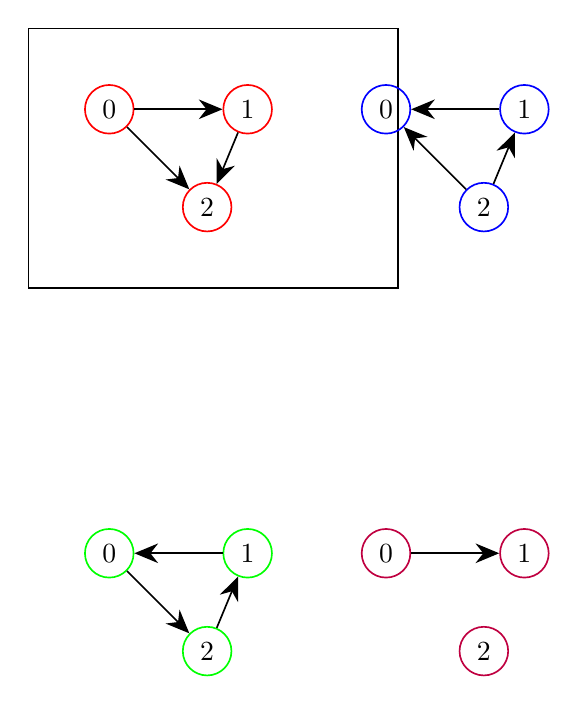
\begin{tikzpicture}[node distance=5em,->,
				-{Stealth[scale=1.5,angle'=45]},semithick]
				\tikzset{state/.style={fill=none, draw=red, text=black,
					shape=circle}}
				\node[state] (0) {0};
				\node[state] (1) [right of=0] {1};
				\node[state] (2) [below right of=0] {2};
				\path	(0) edge node {} (1)
						(0) edge node {} (2)
						(1) edge node {} (2);
				\draw ($(0.north west)+(-.8,.8)$) rectangle ($(2.south 
					east)+(2.2,-.8)$);

				\tikzset{state/.style={fill=none, draw=blue, text=black,
					shape=circle}}
				\node[state] (3) [right of=1] {0};
				\node[state] (4) [right of=3] {1};
				\node[state] (5) [below right of=3] {2};
				\path 	(5) edge node {} (3)
						(5) edge node {} (4)
						(4) edge node {} (3);

				\tikzset{state/.style={fill=none, draw=green, text=black,
					shape=circle}}
				\node[state] (6) [below=5cm of 0] {0};
				\node[state] (7) [right of=6] {1};
				\node[state] (8) [below right of=6] {2};
				\path 	(6) edge node {} (8)
						(8) edge node {} (7)
						(7) edge node {} (6);
					
				\tikzset{state/.style={fill=none, draw=purple, text=black,
					shape=circle}}
				\node[state] (9) [right of=7] {0};
				\node[state] (a) [right of=9] {1};
				\node[state] (b) [below right of=9] {2};
				\path 	(9) edge node {} (a);

			\end{tikzpicture}
		\end{center}
	\end{posterboxtitle}
	}	


	%\begin{posterboxtitle}{Model}
	%	\noindent\textbf{First Layer}
	%	\begin{itemize}
	%		\item Accepts spike-time raster plots for each of \textit{n} neurons
	%		\item Converts to $(d \times n^2)$ matrix, with each 
	%			\textit{d}-vector representing one potential edge
	%		\item Figure here
	%	\end{itemize}
	%	\noindent\textbf{Locality Layer}
	%	\begin{itemize}
	%		\item Accepts data from the first layer
	%		\item Incoporates data from potentially adjacent edges into the 
	%			calculation of the existence of a given edge
	%		\item Figure here
	%	\end{itemize}
	%	\noindent\textbf{Final Layer}
	%	\begin{itemize}
	%		\item Converts output from locality layer into $(n \times n)$ 
	%			adjacency matrix
	%		\item figure also here
	%	\end{itemize}
	%\end{posterboxtitle}

	%\begin{posterboxtitle}{Trained Model Weights}
	%	\begin{center}
	%		\textbf{First Layer Weights}\\
	%		\vspace{1em}
	%		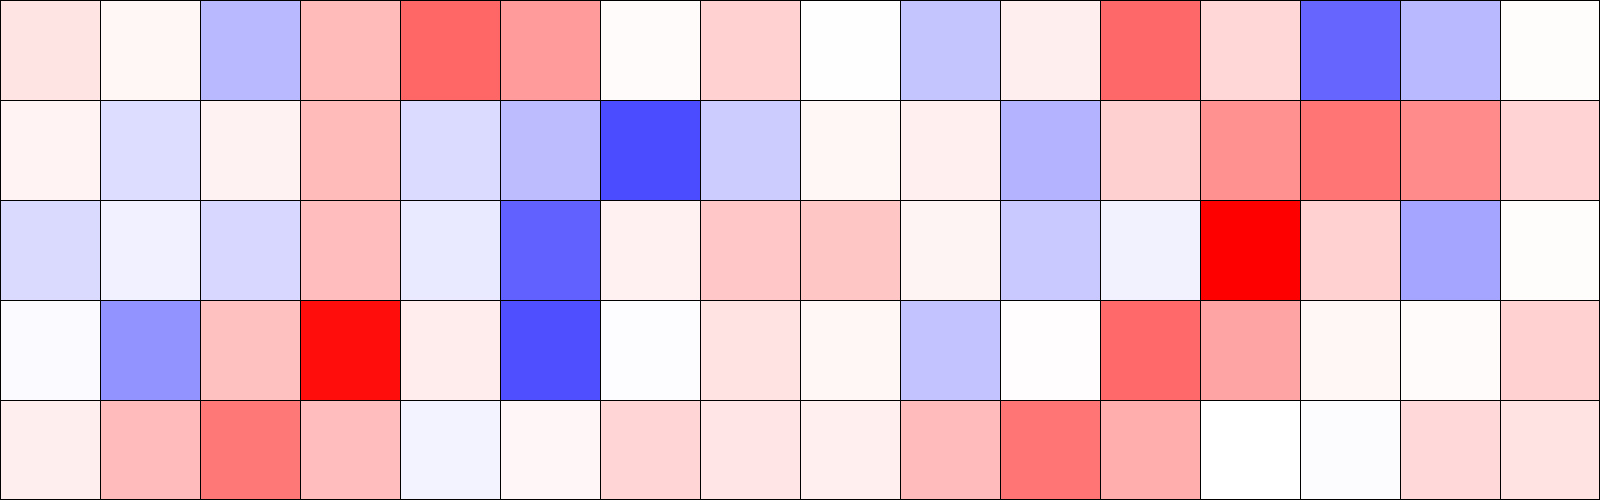
\includegraphics[width=.65\textwidth]{fullRun/0_py/layer0/weights.png}\\
	%		(max: 1.44)\\
	%		\vspace{1em}
	%		\textbf{Second Layer Weights}\\
	%		\vspace{1em}
	%		\begin{tikzpicture}
	%			\node (in_cap) {Input Weights};
	%			\node (in) [below=1em of in_cap] 
	%				{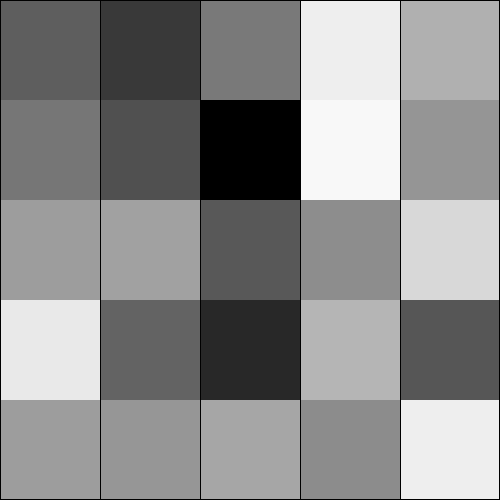
\includegraphics[width=.2\textwidth]{fullRun/0_py/layer1/weights_in.png}};
	%			\node (out) [right=1em of in] 
	%				{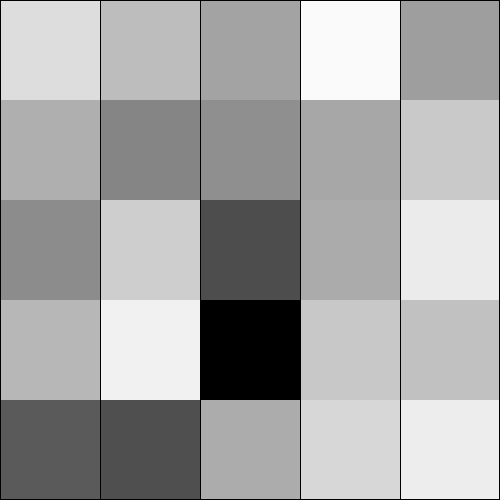
\includegraphics[width=.2\textwidth]{fullRun/0_py/layer1/weights_out.png}};
	%			\node (out_cap) [above=1em of out] {Output Weights};

	%			\node (in_max) [below=5pt of in] {(max: -1.24)};
	%			\node (out_max) [below=5pt of out] {(max: -1.65)};
	%			\node (total) [right=1em of out] {
	%					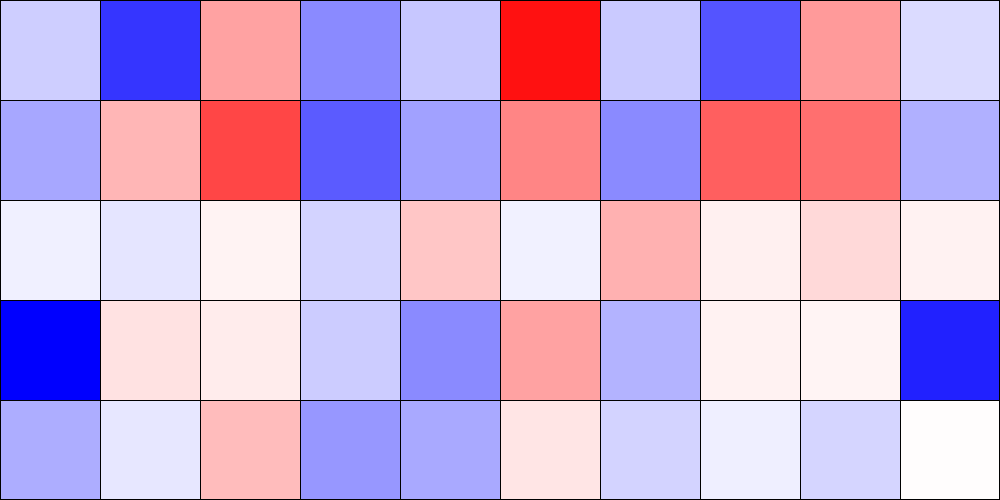
\includegraphics[width=.4\textwidth]{fullRun/0_py/layer1/weights_f.png}
	%				};
	%			\node (total_cap) [above=1em of total] {Combination Weights};
	%			\node (total_max) [below=5pt of total] {(max: -1.01)};
	%		\end{tikzpicture}
	%		\textbf{Final Layer Weights}\\
	%		\vspace{1em}
	%		\begin{tikzpicture}
	%			\node (w_f) {
	%				
\includegraphics[width=.2\textwidth]{fullRun/0_py/layerf/weights.png}};
	%			\node (max) [right=1em of w_f] {(max: 7.31)};
	%		\end{tikzpicture}

	%	\end{center}

	%\end{posterboxtitle}

	%\begin{posterboxtitle}{Trained Model Operation}
	%	\begin{center}
	%		\begin{tikzpicture}
	%			\node (input) {
	%					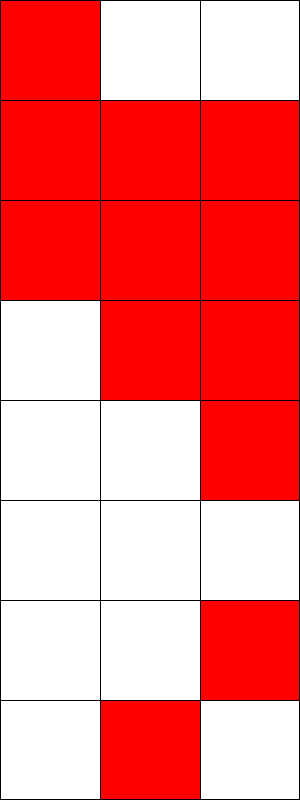
\includegraphics[width=.105\textwidth]{fullRun/0_py/input.png}
	%				};
	%			\node (input_label) [above=1em of input] {Input};
	%			\node (layer0) [right=1em of input] {
	%				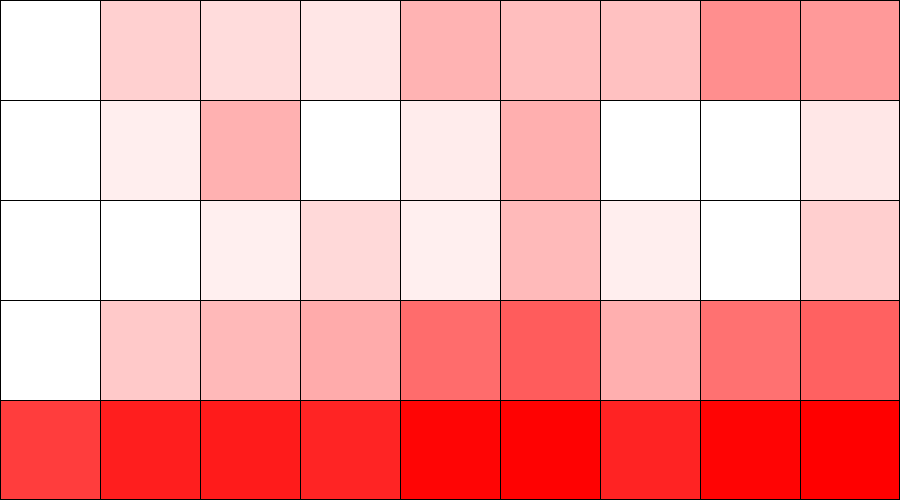
\includegraphics[width=.5\textwidth]{fullRun/0_py/layer0/4out.png}};
	%			\node(layer0_label) [above=1em of layer0] {Layer 1 Output};
	%		\end{tikzpicture}
	%	\end{center}
	%\end{posterboxtitle}

	\begin{posterboxtitle}{Results}
		\noindent It became clear that our architecture:
		\begin{enumerate}
			\item can reconstruct network structure from spiking data with 
				relative ease for small \textit{n}
			\item can reconstruct networks that it has no training on, as long 
				as the network is similar in nature to the training data
			\item learns features of the networks it analyzes: a model trained 
				only on connected graphs will always predict at least one 
				connection at each neuron
			\item on small \textit{n} ultimately does no better than a simpler 
				model
		\end{enumerate}
		Preliminary results on much larger networks ($n > 50$) suggest a great 
		leap in efficacy relative to a simple benchmark model; this falls into 
		the future work category.
	\end{posterboxtitle}

	{\boxtitlecolor{Lavender}
	\begin{posterboxtitle}{Future Work}
		\noindent While our results demonstrate that our algorithm can 
		reconstruct networks, they do not show that the locality operations 
		produce any more useful data than our benchmark model. Based on 
		preliminary results, demonstrating this would require:
		\begin{enumerate}
			\item Testing on a large scale - the small-\textit{n} networks we 
				used do not present a difficult enough problem to make clear 
				whether or not our model has an advantage over simpler 
				architectures
			\item Testing on highly structured vs. random networks - if our 
				model is indeed learning local features to help reconstruction, 
				it should be more effective when used on highly structured 
				networks than on random networks
		\end{enumerate}
		After completing those benchmarks, and assuming positive results, the 
		next step would be to refine the algorithm and apply it to more 
		realistic data, which is generally more complex and noisy than the data 
		used here.\\
	\end{posterboxtitle}
}


\end{posterbard}

\end{document}
